\section{Design}
\subsection{Architettura}

In fase di progettazione è stato scelto di adottare il pattern architetturale MVC, traendone quindi tutti i suoi vantaggi, principalmente che model e controller rimangono praticamente uguali a prescindere dalla view utilizzata. Infatti, è stato scelto nella view di usare il pattern Strategy con delle interfacce generiche per i singoli componenti che potranno perciò adottare qualsiasi GUI framework. Per passare, per esempio da Swing a JavaFX basterebbe solo sostituire le implementazioni delle interfacce presenti nella parte di view. Ogni modulo del pattern Model-View-Controller ha quindi una propria organizzazione e scopo:
\begin{itemize}
    \item Nella parte di model sono state definite le entità che modellano: tessere (tile), seguaci (meeple), strutture (gameset) e giocatori (player). Esse vengono instanziate e gestite dal controller.
    \item Nella parte di view è presente un componente principale, la UserInterface, che si occupa di gestire tutti i componenti grafici e di renderli visibili all'utente quando necessario. Quest'ultima si occupa anche di fornire ai vari componenti, ognuno con uno scopo ben preciso, l'accesso regolarizzato alla parte di controller. Nella maggior parte dei casi questi componenti sono annidati l'uno dentro l'altro.
    \item La parte di controller si occupa della gestione della partita e di propagare sul model i risultati delle azioni compiute dall'utente attraverso la view.
\end{itemize}
Siccome ad ogni modifica di stato della partita, il Controller notifica le UserInterface collegate ad esso, è possibile giocare alla stessa partita contemporaneamente tramite varie interfacce utente aggiungendole tutte allo stesso controller. Queste possono essere diverse tra loro e di qualsiasi tipo, per esempio: Web, CLI o come nel nostro caso, GUI.


% TODO spostare
% (parlare del Mediator che gestisce la doppia referenza e del Mutable/non Mutable, insieme a Factory, Builder e Strategy)
% (parlare del fatto che la UserInterface è l'interfaccia principale che pilota tutto, del Composition over inheritance e delle matrioska di Component/JPanel nella quale vengono diffusi aggiornamenti (update) ed informazioni)
%  Per permettere l'aggiunta di nuovi tipi di seguaci con meccaniche diverse abbiamo adottato il pattern \textit{strategy}, lo stesso principio vale anche per tessere e strutture. Per facilitare la generazione di diverse tessere, che condividono la medesima rappresentazione grafica, abbiamo utilizzato il pattern \textit{factory method} che definisce per ognuna di esse un metodo per la creazione. Il medesimo design pattern è stato utilizzato anche per la creazione delle diverse strutture. Siccome le singole tessere di loro contengono già delle strutture al loro interno
\subsection{Design dettagliato}

\subsection*{Mauro Pellonara}

\subsection*{Alessandro Martini}
\subsubsection*{Definizione di operazioni che vengono utilizzati su GameSet differenti}
\begin{figure}[ht]
    \centering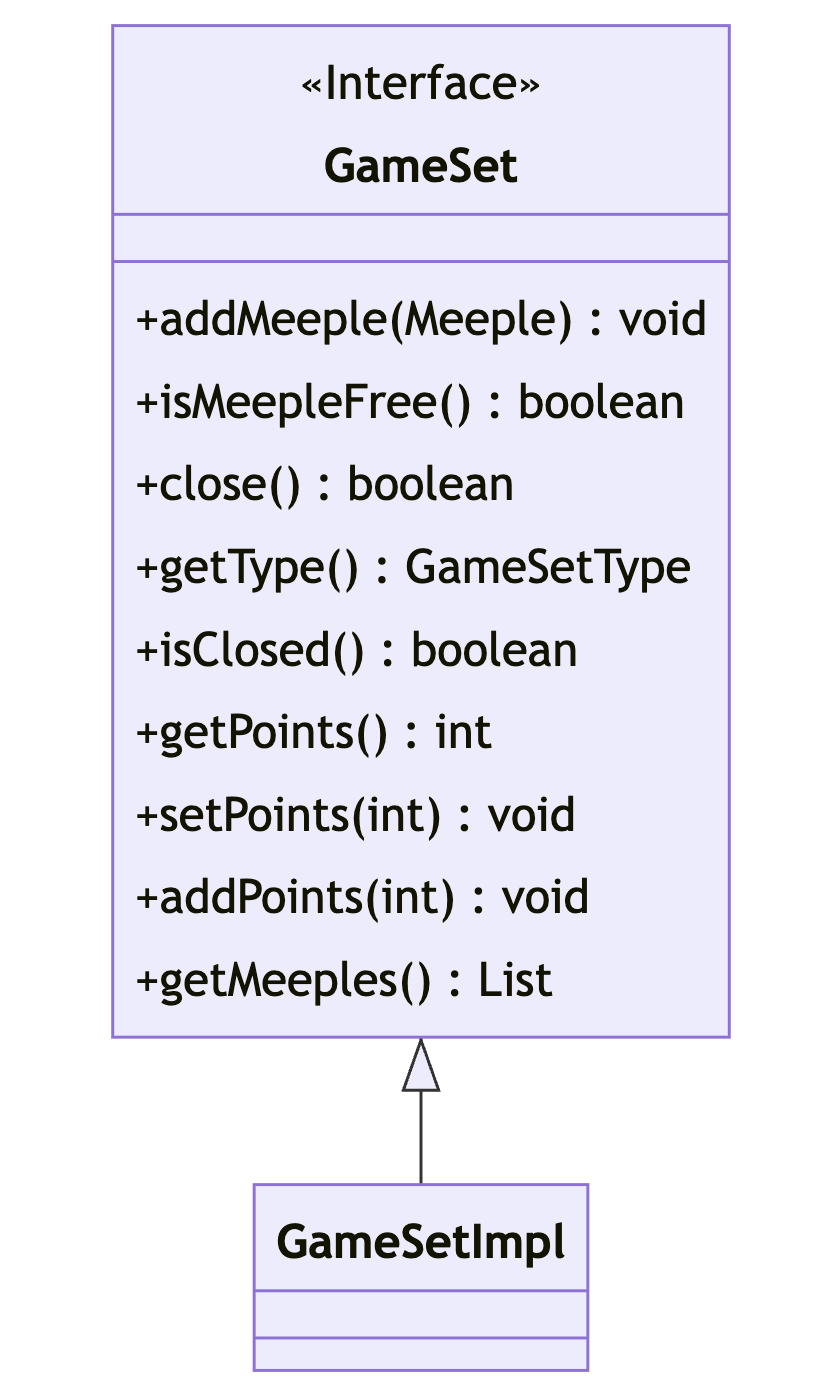
\includegraphics[scale=.4]{images/gameset.png}
    \caption{Rappresentazione UML dell'applicazione del pattern Strategy per il GameSet e GameSetImpl}
\end{figure}
\paragraph{Problema:}
A ogni GameSet, va assegnato il relativo punteggio, il controllo se vi sono meeple presenti e la possibilità di piazzarli, la tipologia del GameSet e infine se è ancora aperto o chiuso.
\paragraph{Soluzione:}
La classe GameSetImpl implementa lo Strategy pattern, avendo come riferimento GameSet che serve come strategy per la gestione delle informazioni di ogni singolo GameSet.

\subsubsection*{Creazione di più GameSet con tipologie differenti}
\begin{figure}[ht]
    \centering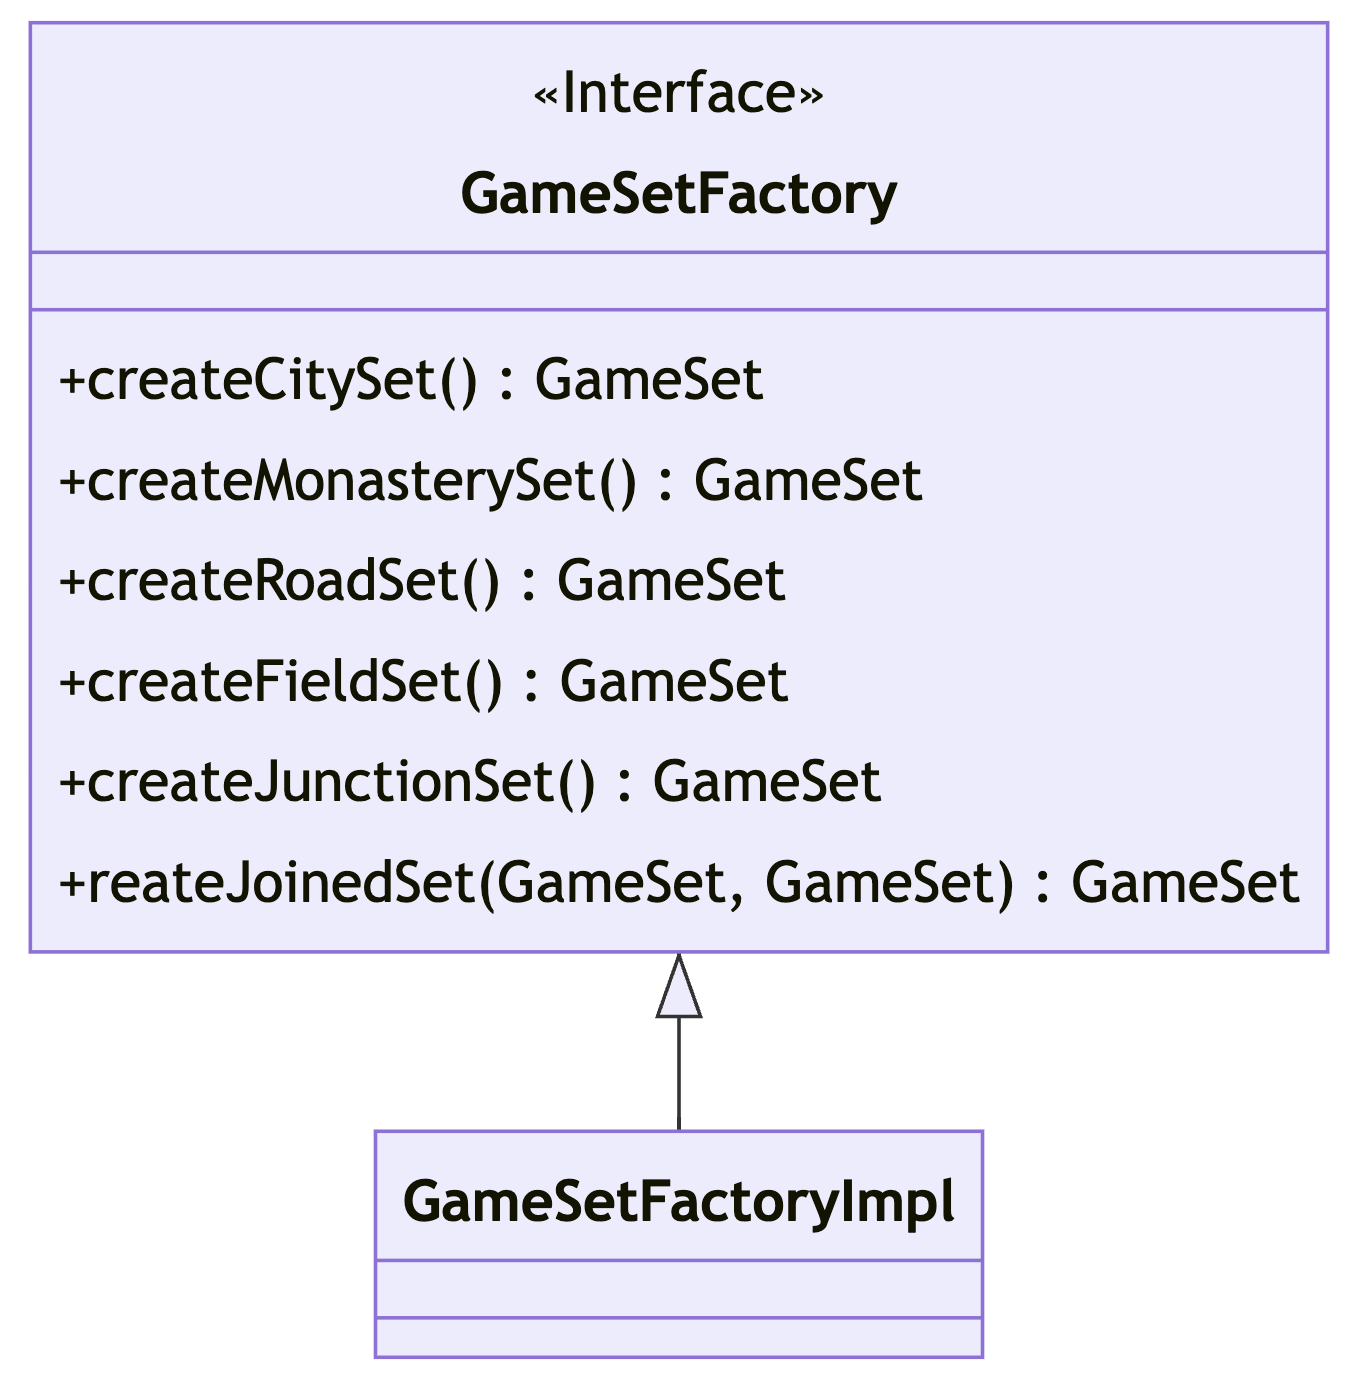
\includegraphics[scale=.3]{images/gamesetfactory.png}
    \caption{Rappresentazione UML dell'applicazione del pattern Strategy per il gamesetfactory e GameSetFactoryImpl}
\end{figure}

\paragraph{Problema:}
Possono esistere più GameSet con informazioni differenti e relativi punteggi assegnati, in aggiunta si devono gestire l'unione di due GameSet.
\paragraph{Soluzione:}
La classe GameSetFactoryImpl implementa lo Strategy pattern, avendo come riferimento GameSetFactory che serve come strategy per la creazione di nuovi GameSet.

\subsubsection*{Creazione di più BasicComponent con caratteristiche differenti}
\begin{figure}[ht]
    \centering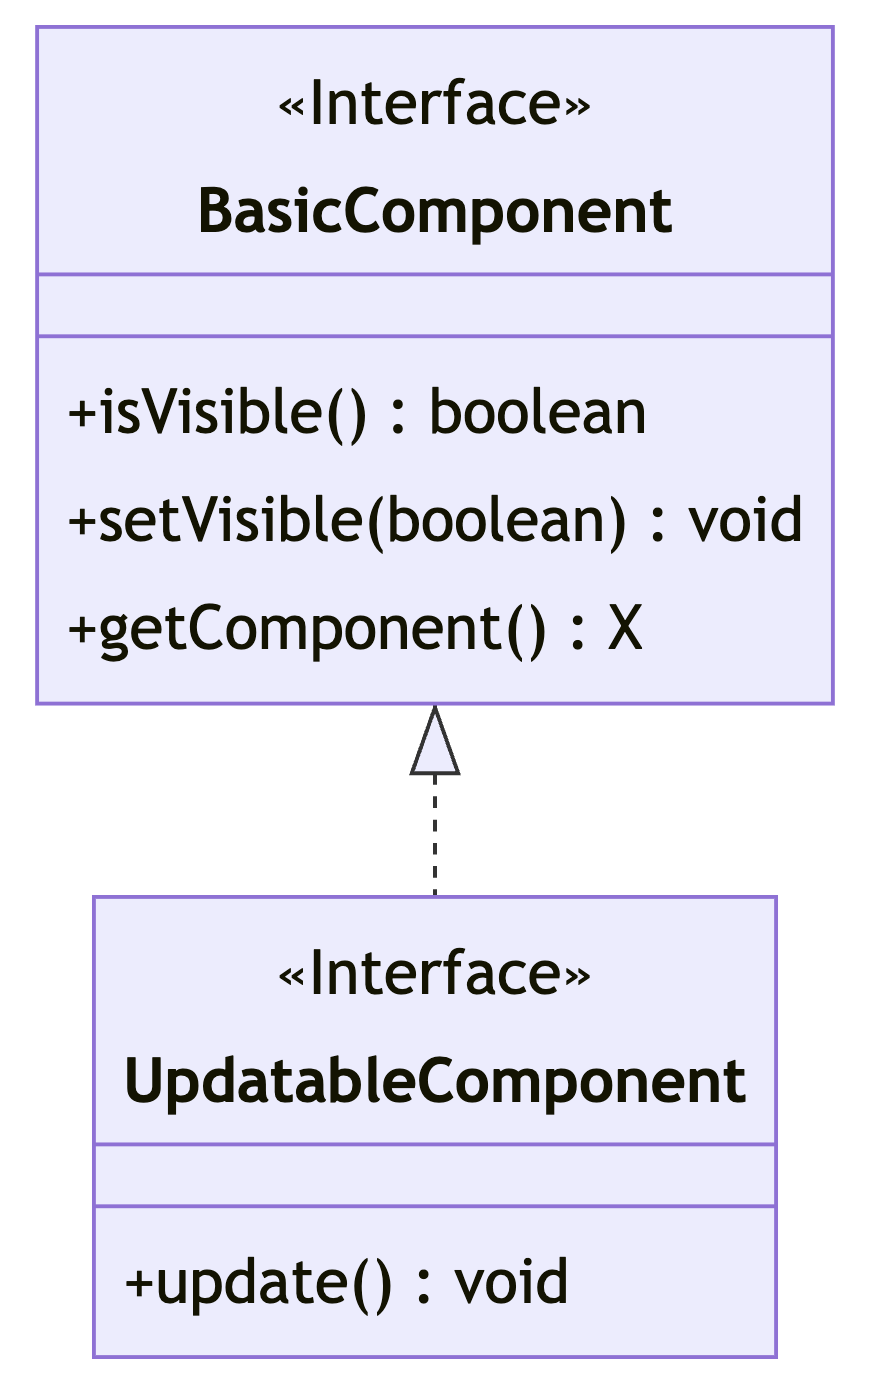
\includegraphics[scale=.5]{images/basiccomponent.png}
    \caption{Rappresentazione UML dell'applicazione del pattern Strategy per la classe interfaccia BasicComponent, che viene estesa da TileButton, a sua volta implementato da TileButtonImpl}
\end{figure}

\paragraph{Problema:}

\paragraph{Soluzione:}


\subsection*{Davide Speziali}

\subsection*{Samuele Giancarli}


Problema: piazzamento di una tessera



ecco cosa fa il getCurrentTile:

\begin{itemize}
\item va a verificare che la posizione selezionata non fosse stata già occupata da un’altra tessera, in caso negativo ritorna false
\item va a verificare che esista almeno una tile neighbour, in caso negativo ritorna false
\item va a verificare per ogni tile neighbour che la totalità delle section adiacenti alla current tile siano dello stesso tipo
\item solo dopo aver controllato ogni section di ogni neighbour e aver appurato che la current tile sia piazzabile allora: setPosition(position)
\item a questo punto ad ogni neighbour dovranno essere impostate a closed le section connesse con la current tile. La stessa cosa verrà fatta per le section della current tile connesse a quelle di un neighbour.
\subitem la struttura del ciclo è la stessa di quello precedente, ma è solo grazie al completamento del ciclo precedente che si avrà la sicurezza di poter impostare tutte le section a closed
\item (??????) solo a questo punto sarà possibile unire i gameset della tile corrente con quelli delle tile già presenti
\end{itemize}
